\section{Paper 8}
\subsection{\emph{"Visual Object Tracking via Multi-Stream Deep Similarity Learning Networks"}}

\begin{frame}{INTRODUCTION}
    The goal of visual tracking systems is to be able to obtain the position of 
    the tracked target even in subsequent frames. The problems to be solved 
    are those of occlusion, background clutter, illumination variations, 
    deformation etc. The following paper uses a model that compares 
    similarities and is trained offline in order to predict the patch present in 
    the next frame. The method, thanks to the use of the relative distance, 
    is robust in the presence of phenomena that introduce the so called 
    \emph{distractors}.
\end{frame}

\begin{frame}{RELATED WORK}
    Some methods train a CNN offline while the test is done online. Unfortunately, 
    these models are not fast. Other models instead if they fail a first 
    time, then they will always fail until the target returns to the search region. 
    Other methods \footfullcite{0893551129} \footfullcite{0893551134} search for the target template in subsequent frames 
    in the same position, obtaining better performance than methods based on 
    similarity but nevertheless are not robust to distracting elements. The proposed 
    method instead takes into account both the \emph{background patches} and 
    the \emph{target template patches} in order to make comparisons on similarities.
\end{frame}

\begin{frame}{METHODS - EMDSLT Architecture}
    The proposed framework, called Ensemble Multi Deep Stream Similarity 
    Learnining Tracking (EMDSLT), is composed of some networks. Those 
    in blue are fully-convolutional networks while those in red are useful for 
    re-verification and re-detection operations, responsible for recovery from 
    failures and the template updating.
    \begin{figure}[h!]
        \centering
        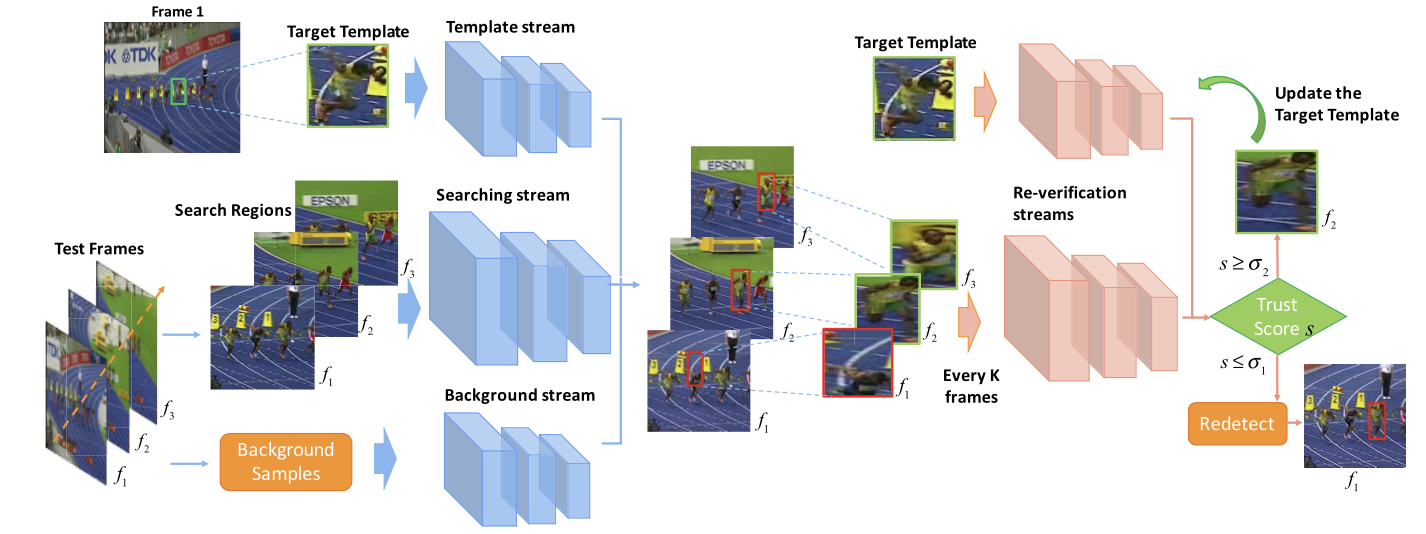
\includegraphics[width = \linewidth]{images/paper8/EMDSLT.png}
        \centering
        \caption{The EMDSLT framework.}
        \label{fig:EMDSLT}
    \end{figure}
\end{frame}

\begin{frame}{METHODS - Streams}
    The target template \emph{T}, the patches $X_i^+$ positive and the background patches $B_{i-1,j}$, are extracted from the first convolutional networks. These elements are useful for calculating the \emph{Template-Searching-Background Loss} (TSB).
    \begin{figure}[h!]
        \centering
        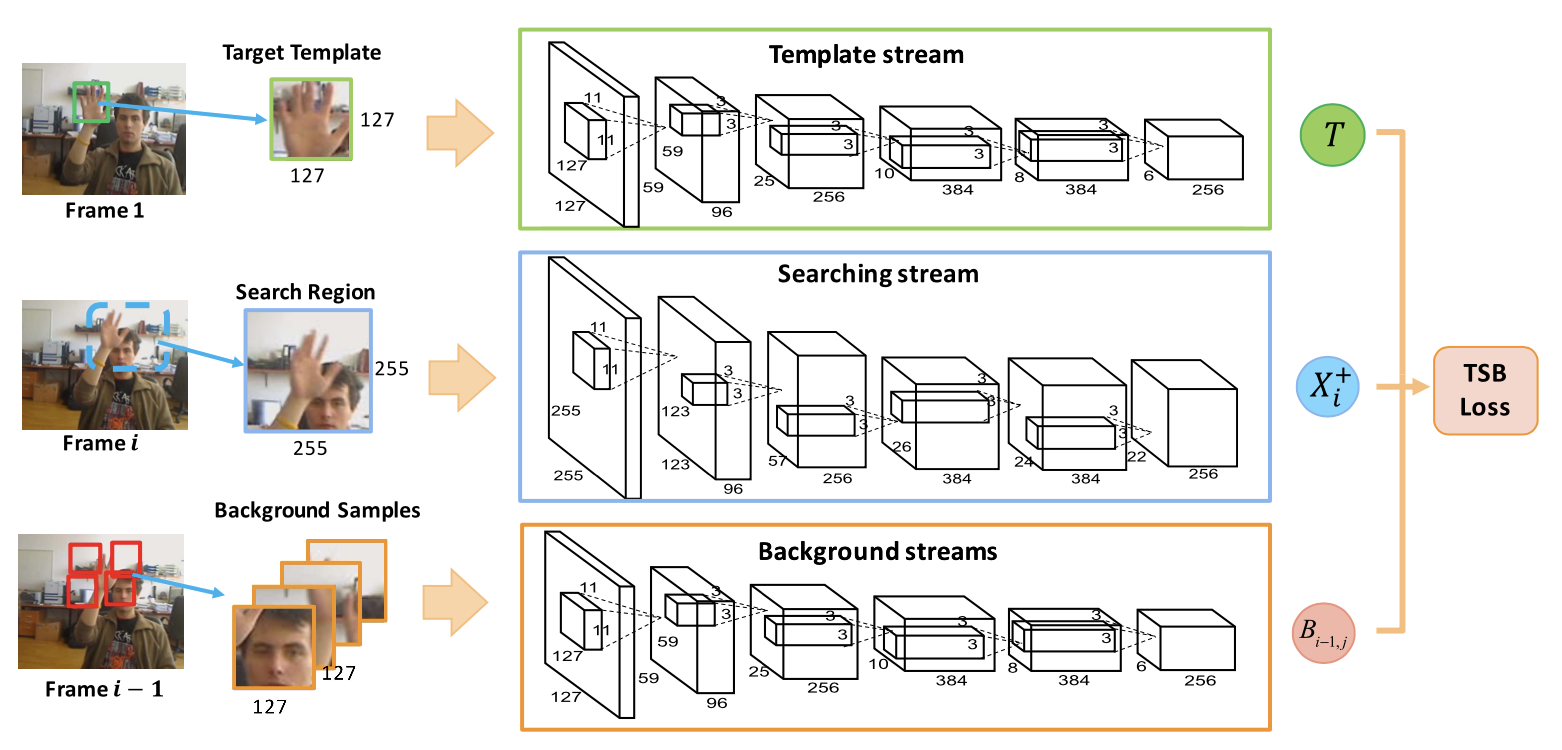
\includegraphics[width = \linewidth]{images/paper8/streams.png}
        \centering
        \caption{Multi Deep Streams}
        \label{fig:streams}
    \end{figure}
\end{frame}

\begin{frame}{METHODS - \emph{Template-Searching-Background Loss} (TSB)}
    The use of the Template-Searching-Background (TSB), allows to use the 
    background patches to train the model. This method helps to minimize 
    the relative distance $d(\cdot)$ (\ref{distanceFunc}) which translated into other words means 
    bringing the target template closer to the $X_i^+$ samples and at the same 
    time moving the background distractors $B_i$ away from the positive 
    sample.
    \begin{minipage}{\linewidth}
        \centering
        \begin{minipage}{0.45\linewidth}
            \begin{block}{RELATIVE DISTANCE}
                \begin{equation}\label{distanceFunc}
                    d_i=\sum^M_{j=1} D(T, X_i) - D(X_i, B_{i-1,j})
                \end{equation}
            \end{block}  
        \end{minipage}
        \hspace{0.05\linewidth}
        \begin{minipage}{0.47\linewidth}
            \begin{figure}[h!]
                \centering
                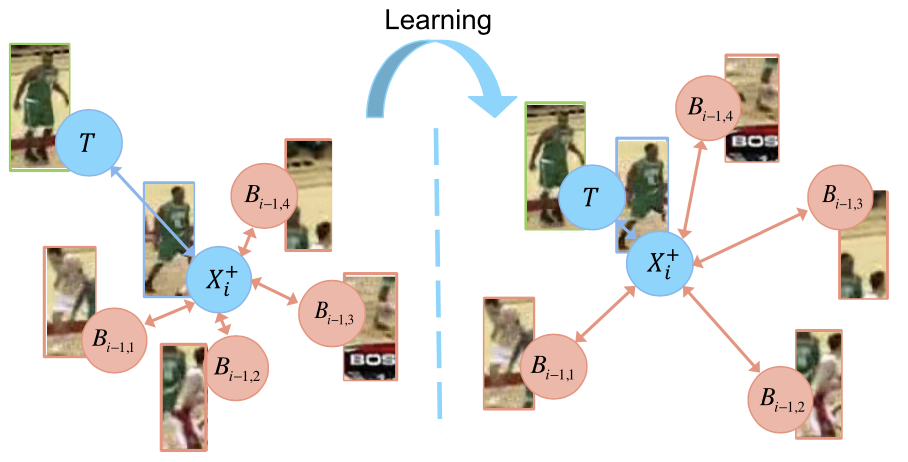
\includegraphics[width =\linewidth]{images/paper8/TSB.png}
                \centering
            \end{figure}
        \end{minipage}
    \end{minipage}
\end{frame}

\begin{frame}{METHODS - Tracking With Updating}
    To evaluate the correspondence of an $X_i^+$ patch, a \emph{Trust Score s} is calculated. The score $s$ will be compared with two thresholds $\sigma_1$ and $\sigma_2$.
    If $s\leq\sigma_1$ then a new positive patch $X{'}_i^+$, and consequently a new score $s'$, will be recalculated which will be replaced with the previous patch $X_i^+$ when $s'\geq\sigma_1$.
    If $s\geq\sigma_2$ then update the target template $T$ with $X_i^+$.
    \begin{equation}\label{distanceFunc}
        X_i = \argmin_{X_{i,k} \in S_i}d(T,X_{i,k}, \{B_{i-1,j}\}^M_{j=1})
    \end{equation}
    \begin{equation}\label{newX}
        X'_i = \argmax_{X_{i,k} \in S_i}m(T,X_{i,k})
    \end{equation}
\end{frame}

\begin{frame}{EXPERIMENTS}
    The experiments were conducted on four different types of datasets: 
    OTB-2013, OTB-100, VOT-2015 and VOT-2016. The metrics used to 
    evaluate the performance of all existing methods, including the one 
    proposed, are accuracy, Area-Under-the-Curve (AUC), 
    Expected-Average-Overlap (EAO) and robustness.
    \begin{figure}[h!]
        \centering
        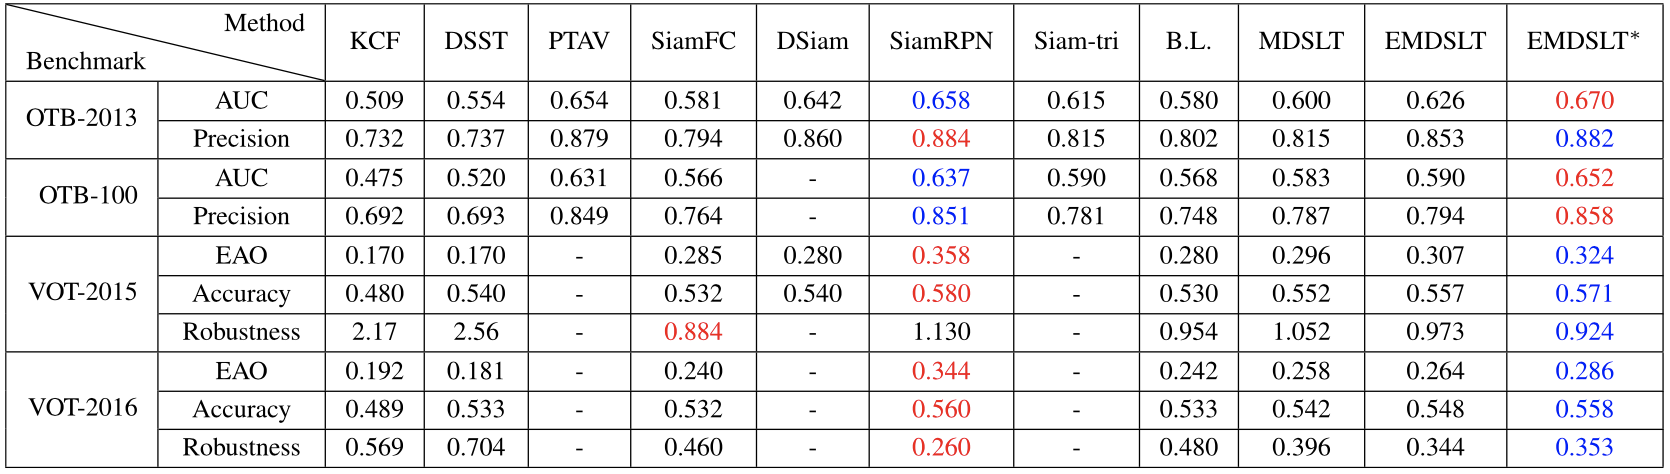
\includegraphics[width = \linewidth]{images/paper8/metrics.png}
        \centering
    \end{figure}
\end{frame}

\begin{frame}{EXPERIMENTS - AUC score on distractors}
    Target tracking can be onerous when there are elements such as 
    distractors in the scene. These lead most trackers to fail. The 
    re-verification and re-detecting operations were essential to reduce this 
    problem. In the table, the values in blue are the highest and are obtained 
    from the best method, while those in red are placed in second position.
    \begin{figure}[h!]
        \centering
        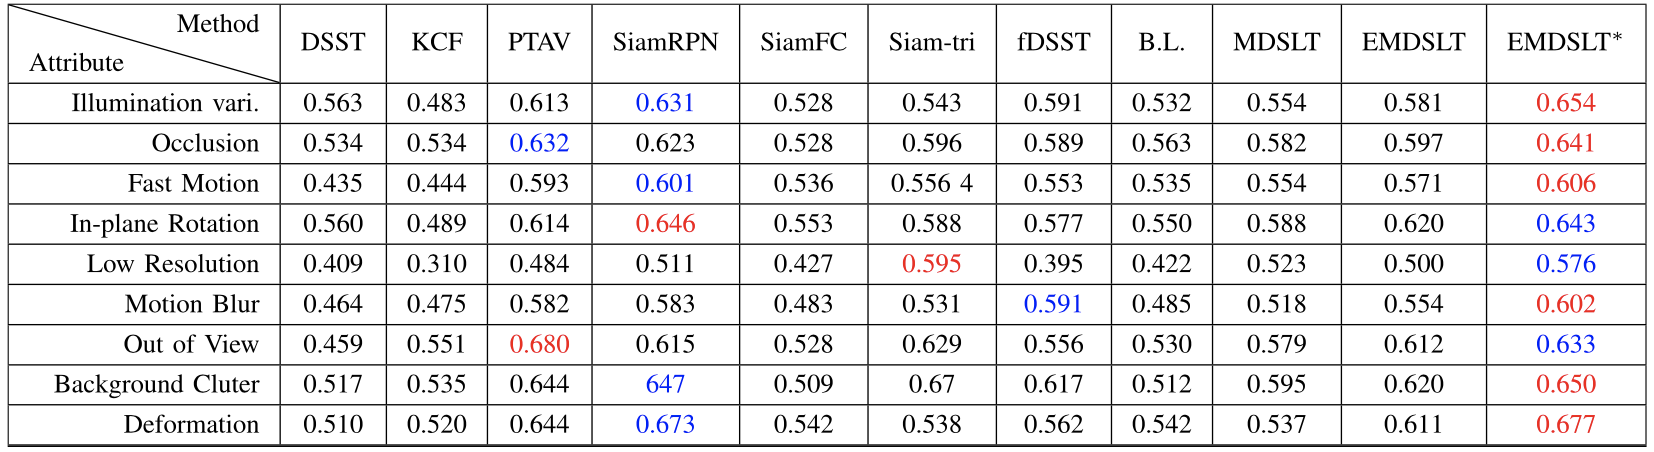
\includegraphics[width = \linewidth]{images/paper8/AUC.png}
        \centering
    \end{figure}
\end{frame}

\begin{frame}{CONCLUSION}
    The proposed framework, from the results obtained in the benchmarks, seems 
    to be the best. The achievement of these results were possible thanks to the 
    integration of a verification and detecting method. The use of the TSB 
    method was fundamental, which, by reducing the relative distance between 
    the various patches, allowed for good model learning.
\end{frame}